
\documentclass{article} % Don't change this

\usepackage[english]{babel}
\usepackage[utf8]{inputenc}
\usepackage[margin=1.2in]{geometry}
\usepackage{amsmath}
\usepackage{amsthm}
\usepackage{amsfonts}
\usepackage{multirow}
\usepackage{amssymb}
\usepackage{multicol}
\usepackage{booktabs}
\usepackage[usenames,dvipsnames]{xcolor}
\usepackage{graphicx}
\usepackage[siunitx]{circuitikz}
\usepackage{tikz}
\usepackage{lscape}
\usepackage[colorinlistoftodos, color=orange!50]{todonotes}
\usepackage{hyperref}
\usepackage[authoryear]{natbib}
\setcitestyle{authoryear,open={(},close={)}}
\usepackage{fancybox}
\usepackage{epsfig}
\usepackage{soul}
\usepackage{listings}
\usepackage{subcaption}
\lstset{language=[90]Fortran,
  basicstyle=\ttfamily,
  keywordstyle=\color{red},
  commentstyle=\color{green},
  morecomment=[l]{!\ }% Comment only with space after !
}

\usepackage{booktabs}
\setlength{\marginparwidth}{3.4cm}

\usepackage[default]{sourceserifpro}
\usepackage[T1]{fontenc}



%#########################################################

%To use symbols for footnotes
\renewcommand*{\thefootnote}{\fnsymbol{footnote}}
\newcommand{\tp}{\texttt}
%To change footnotes back to numbers uncomment the following line
%\renewcommand*{\thefootnote}{\arabic{footnote}}

% Enable this command to adjust line spacing for inline math equations.
% \everymath{\displaystyle}

\title{\raggedright
\normalfont \normalsize 
\huge Message-Passing Programming: 2-D Image Recomposition Coursework \\[1em]
\normalsize \normalfont Jack Tyler: 27513556 \\
\rule{\linewidth}{.5pt}  \\[6pt]
}
\date{27 May, 2019}

\begin{document}

\maketitle

In the early days of computing, computational power progressed at an alarming rate; constant field scaling meant that transistors could be fabricated smaller and smaller, allowing them to use less power, and increasing their clock speed.
However, transistor manufacture has hit a physical limit for scaling \citep{Mcfarland1995}, and increasing the clock speed any further would require highly capable cooling solutions impractical for use.
As a result, processor companies have had to find other methods to speed up computer processors to keep computational power, and Moore's Law, advancing.
Perhaps most prominent is the introduction of distributed parallelism, where multiple processor units, which otherwise operate asynchronously and independently, may communicate while performing some task.

This type of parallelism is one of the most common implementations currently used in high-performance computing to decrease program execution time.
However, care must be taken as to data synchronisation occurs between processors: since distributed parallelism does not share memory, data must be explicitly passed between any workers in a pool.

This report investigates the performance of a two-dimensional image re-composition program; in particular, it studies the strong scaling for the program, and analyses several methods of handling file operations. 
This work will also identify many of the limitations and shortcomings in both the parallelisation of the algorithm, and in the analysis method.
Knowledge of the Message-Passing Interface (MPI) standard, parallel computing nomenclature and the implementation of the one-dimensional cartesian topology is assumed in this report.

\section*{Introduction}

Edge detection methods, such as the Sobel-Feldmann operator \citep{sobel} or the Canny method \citep{canny}, are widely used in the fields of image segmentation and computer vision, and many algorithms can often be performed in only several iterations.
However, the inverse operation -- of recreating an image given its edges -- is a more complex process, and often requires a large number of iterations.
With images representing a rectangular compute domain that is readily divisible, image re-composition is a problem that lends itself well to being parallelised.

In the case of this work, let $L\left(u,~v\right)$ be a local co-ordinate system attached to every pixel in an image (noting that a pixel is some value between $0$--$255$, where $0$ represents a fully black pixel and $255$ fully white) with $v$ defined as parallel to the gradient direction. If we then assume that the image has been pre-smoothed and can be associated with some scale-space operator $L\left(x,~y\right)$ then we may define an edge as the zero-crossing of the second derivative of $L$. That is, that we mark a pixel as an edge if the following condition holds:

$$
\frac{\partial^2}{\partial v^2}L = 0
$$

\noindent Similarly, we may perform the inverse operation: knowing the second derivative of some scale-space operator allows us to determine the original value of the pixel; for example, this work uses a Jacobi iterator to approximate the original value of the pixel from the second derivative.

$$
L(x,~y) = \frac{1}{4} \left( L(x+1,~y) + L(x,~y+1) + L(x-1,~y) + L(x,~y-1) - L(x,~y)_{xx}\right)
$$

\section*{Parallelising the Algorithm}

Since this is a continuous problem, it can also be computationally intensive for large images. As a result, the use of MPI and multiple, distributed processors, can decrease program run-time.

\begin{figure}
    \centering
    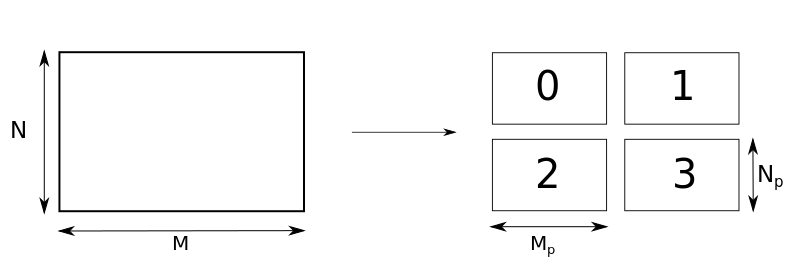
\includegraphics[width=\textwidth]{figures/domain_decomp.png}
    \caption{Two-dimensional domain decomposition used in this work. For some $M$-by-$N$ pixel image, each processor (in this case 4) can be compute an $M_p$-by-$N_p$ chunk of the image.}
    \label{f:domain}
\end{figure}

Consider Figure \ref{f:domain}: for some image that has size $M$-by-$N$ pixels, we may use a domain decomposition technique to split the image in two-dimensions,and each processor may then compute only its local chunk of the whole image.
The MPI standard defines intrinsic routines to perform this Cartesian domain decomposition, and as such, implementing this decomposition is trivial.
However, handling the initial dis-- and re-assembly of the image requires careful implementation.

A description of the parallelisation follows; parallelisation is enabled in the program by compiling with the pre-processor variable PARALLEL2d set equal to $1$ (which may be done with the \texttt{-cpp -DPARALLEL2d} flag on gfortran), which then loads the appropriate library for MPI wrapping subroutines.

$P$ instances of the program are launched via the \texttt{mpirun} or \texttt{aprun} directives, and the MPI communication routines are spawned using the \texttt{MPI\_Init} subroutine.
For portability, all of the MPI routines are wrapped in a library which mimics the serial subroutine calls, and abstracts the parallel modifications from the user.

Also spawned along with the MPI communicator are custom derived data-types and the Cartesian topology in the \texttt{initialise} subroutine call. While the exact structure of the topology is left to MPI to compute, the program will exit with an error should the number of dimensions selected in any direction not be a factor of the size of the image in that direction: this is discussed further in Limitations. 

The derived data-types underpin the successful execution of the software. Four such derived types are defined: two sub-array types, created using the \texttt{MPI\_CREATE\_SUBARRAY} and \texttt{MPI\_CREATE\_RESIZED} subroutines, and two vectors, using the \texttt{MPI\_TYPE\_VECTOR} call.
The sub-arrays enable the use of \texttt{MPI\_SCATTERV} and \texttt{MPI\_GATHERV} routines for the distribution and collection of the original image to all working processors, as in Figure \ref{f:domain}.
The first sub-array type, \texttt{master\_type}, allows for the initial distribution of the image data array onto the working processors.
The second type, \texttt{block\_type}, defines an $(M_p + 2)$-by-$(N_p + 2)$ array of the main $M$-by-$N$ image for each working processor, and is used to gather the individual sub-arrays for each processor.

Two vectors are also created. 
The first is a horizontal vector, which allows for rapid halo swapping between processors aligned above and below each other in the topology, and the second a vertical vector, allows for rapid halo swapping between processors aligned to the left and right of each other in the topology.

Once the initialisation routine has completed, the processor on rank zero in the new, Cartesian communicator reads the input file, which is determined from the appropriate \texttt{fname, M} and \texttt{N} variables in the \texttt{problem\_constants} module file. A call to \texttt{MPI\_SCATTERV} is then performed to send $P$ \texttt{master\_type} sub-arrays to each of the $P$ processors.

The Jacobi iteration then occurs. 
However, each processor has a dependency on data held by other processes. As a result, every iteration of the Jacobi algorithm must be preceded with a series of non-blocking sends and receives to exchange the required data for every processor. Should blocking sends and receives be used, it is possible for the program to hang with nodes unable to progress while they wait for their counterpart -- also waiting to receive -- to send.

In serial versions of the code, this `halo swapping' is not required.

The difference between two most recent iterations is computed every \texttt{check\_int} iterations, adjustable in the \texttt{problem\_constants} module. 
When this value converges to less than the tolerance specified in the same module file, iteration is completed.

After computing their local subset of the image, each processor must then transmit its portion to all other processors to re-assemble the re-composed image.
By using the \texttt{MPI\_GATHERV} subroutine with the \texttt{block\_type} sub-array, the image can be gathered on all processors rapidly.

The zeroth-rank processor will then write the image to the specified output file.

\section*{Testing}

Proper testing of the algorithm is essential to ensuring its functionality.
However, testing parallel applications is often difficult, and this is exacerbated with the time restrictions in this work. 
A suite of tests was performed on the final algorithm, however.

In particular, the results from every image included in the case study were cross-checked and verified against results produced using the sample solutions provided by the EPCC for the workshop, first by eye, and then also using a hybrid Bash/Python testing suite.
The parallel applications were run for each possible case of image -- automated through use of pre-prepared \texttt{problem\_constants} module files -- and the output read into a Python script running OpenCV.
Through use of the \texttt{imread} function, the average value of the solution produced using both the sample solutions and the two-dimensional implementation were checked against each other.
Owing for differences in the results produced by noise, and the additional halo swapping, average values within 5\% of each other were taken to be coherent.

Further tests were performed to check that the program correctly exits in the case of incorrect input: in this case, the program should exit with an \texttt{ERROR STOP} should the incorrect number of processors be specified; the incorrect image dimensions specified; or if the dimensions of the topology are not factors of the dimension of the image, a limitation from the use of rectangular sub-arrays.

\section*{Data Gathering}

The MPI standard provides the \texttt{MPI\_WTIME} subroutine, which can be used in conjunction with the \texttt{MPI\_BARRIER} construct to calculate wall-times for parallel programs. 
In this work, all programs were run ten times and an average time was taken.

Five performance metrics were calculated to measure the performance of the algorithm across different core counts: the time to scatter the image data to all processors; the time to perform the main Jacobi iterations for each thread; the average time to perform the halo swapping routines; and the time required to gather the sub-arrays from the worker processes.
From these timings, the time required per iteration can be computed, and the serial and parallel performance can be identified.

\section*{Results}

The time for iterations to complete is presented in Figure \ref{f:coretime}; note that the heuristics of the time required per iteration is the same, since all images take the same number of iterations to compute (1300), so these have been omitted for the sake of brevity.

\begin{figure}
\begin{subfigure}[b]{.4\textwidth}
    \centering
    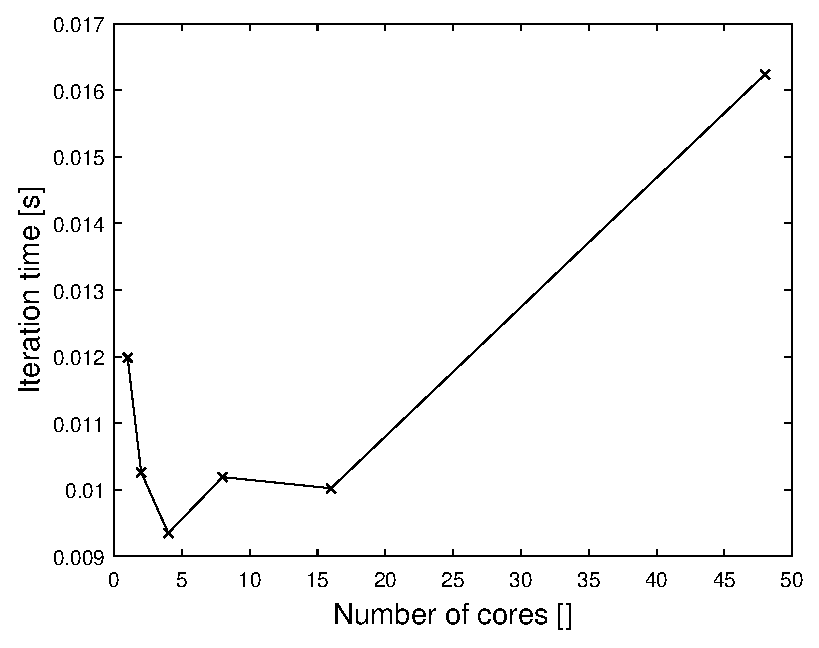
\includegraphics[width=\textwidth]{figures/cores_itertime_198.eps}
    \caption{\texttt{edge198x162.pgm}}
    \label{fig:coretime198}
\end{subfigure}
\hfill
\begin{subfigure}[b]{.4\textwidth}
    \centering
    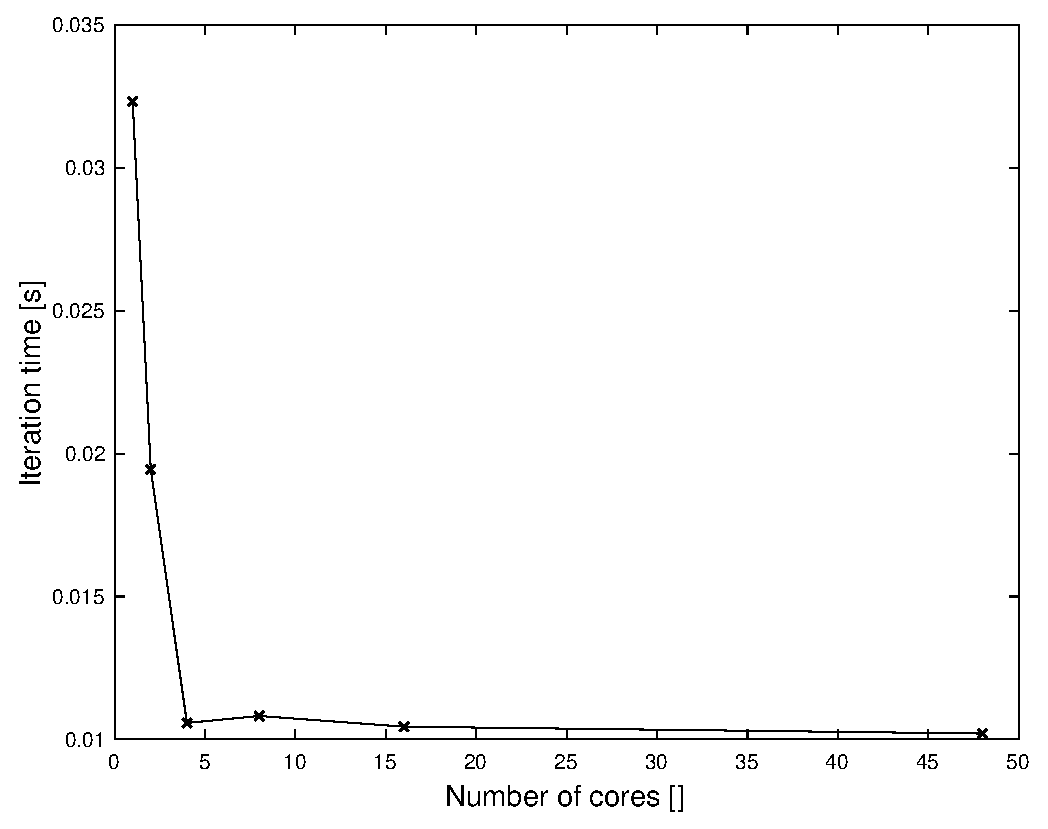
\includegraphics[width=\textwidth]{figures/cores_itertime_256.eps}
    \caption{\texttt{edge256x192.pgm}}
    \label{fig:coretime256}
\end{subfigure}
\begin{subfigure}[b]{.4\textwidth}
    \centering
    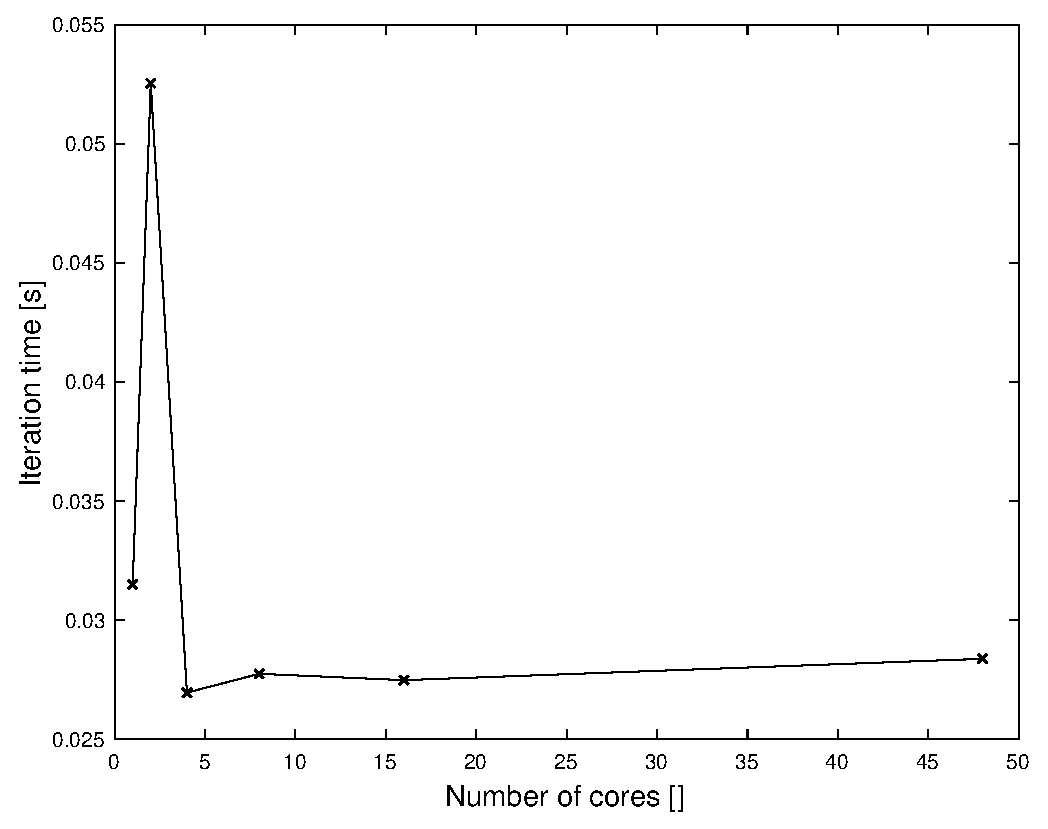
\includegraphics[width=\textwidth]{figures/cores_itertime_384.eps}
    \caption{\texttt{edge512x384.pgm}}
    \label{fig:coretime512}
\end{subfigure}
\hfill
\begin{subfigure}[b]{.4\textwidth}
    \centering
    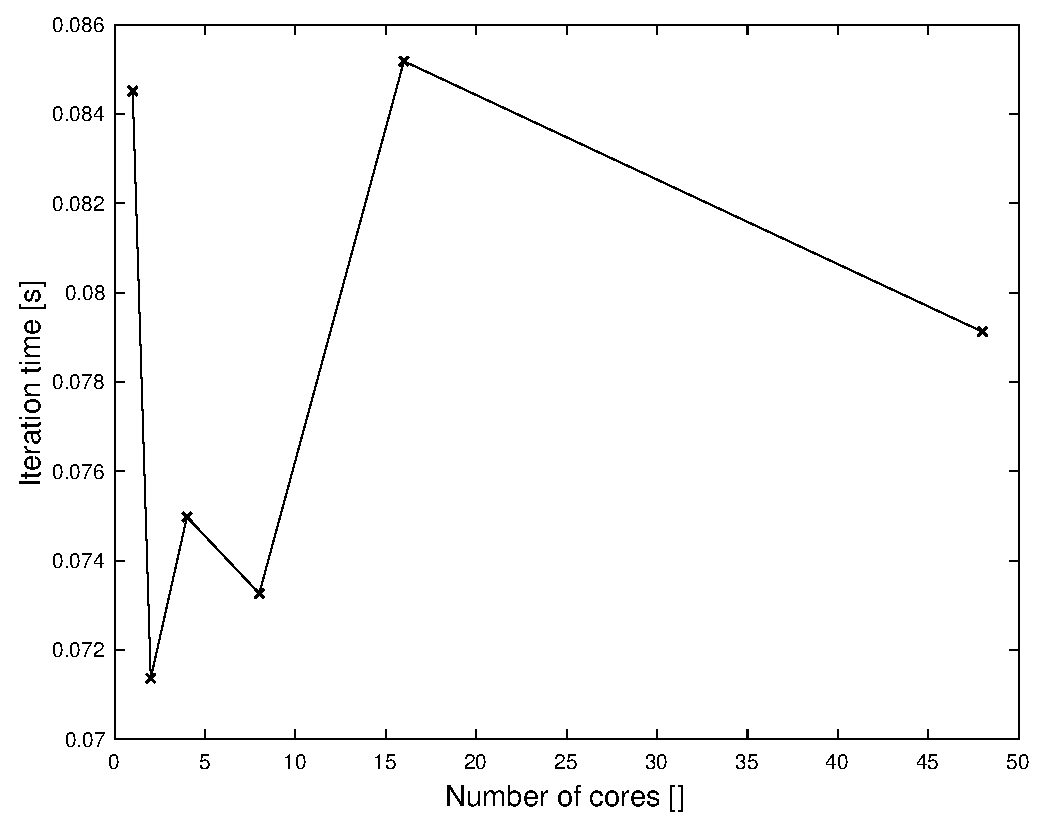
\includegraphics[width=\textwidth]{figures/cores_itertime_768.eps}
    \caption{\texttt{edge768x768.pgm}}
    \label{fig:coretime768}
\end{subfigure}
\caption{Iteration time as a function of the core count for various image sizes. Note that we expect the iteration time to decrease, since the size of the local sub-array for each worker is decreased.}
\label{f:coretime}
\end{figure}

In addition, Figure \ref{f:shares} provides information as to the amount of time the software spends in each portion of its source code.

Figure \ref{f:speedup} shows the strong scaling of the problem; while we appear to gain better than ideal scaling for many of the images, this is as a result of less than ideal performance for a processor count of 1.

% \begin{figure}
% \begin{subfigure}[b]{.4\textwidth}
%     \centering
%     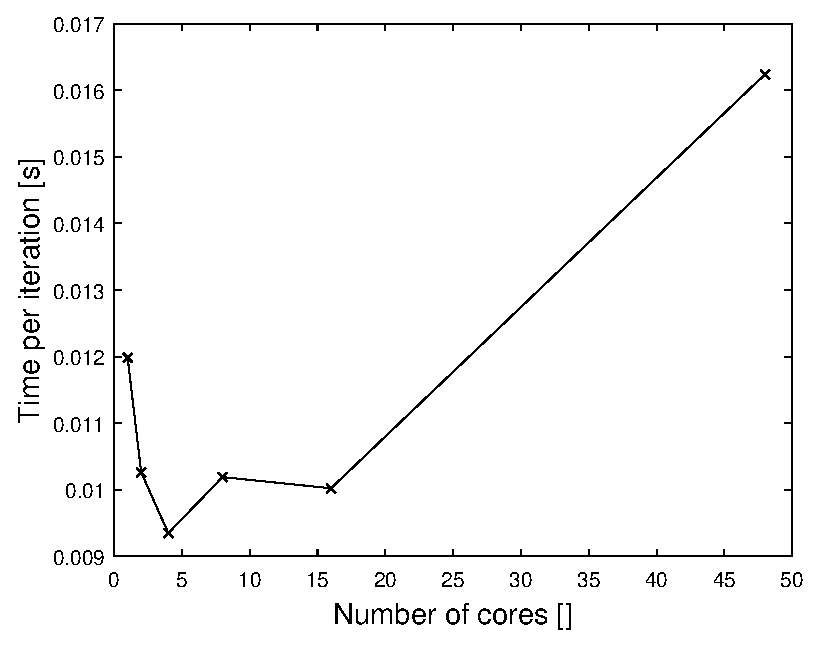
\includegraphics[width=\textwidth]{figures/cores_timeper_198.eps}
%     \caption{\texttt{edge198x162.pgm}}
%     \label{fig:timeper198}
% \end{subfigure}
% \hfill
% \begin{subfigure}[b]{.4\textwidth}
%     \centering
%     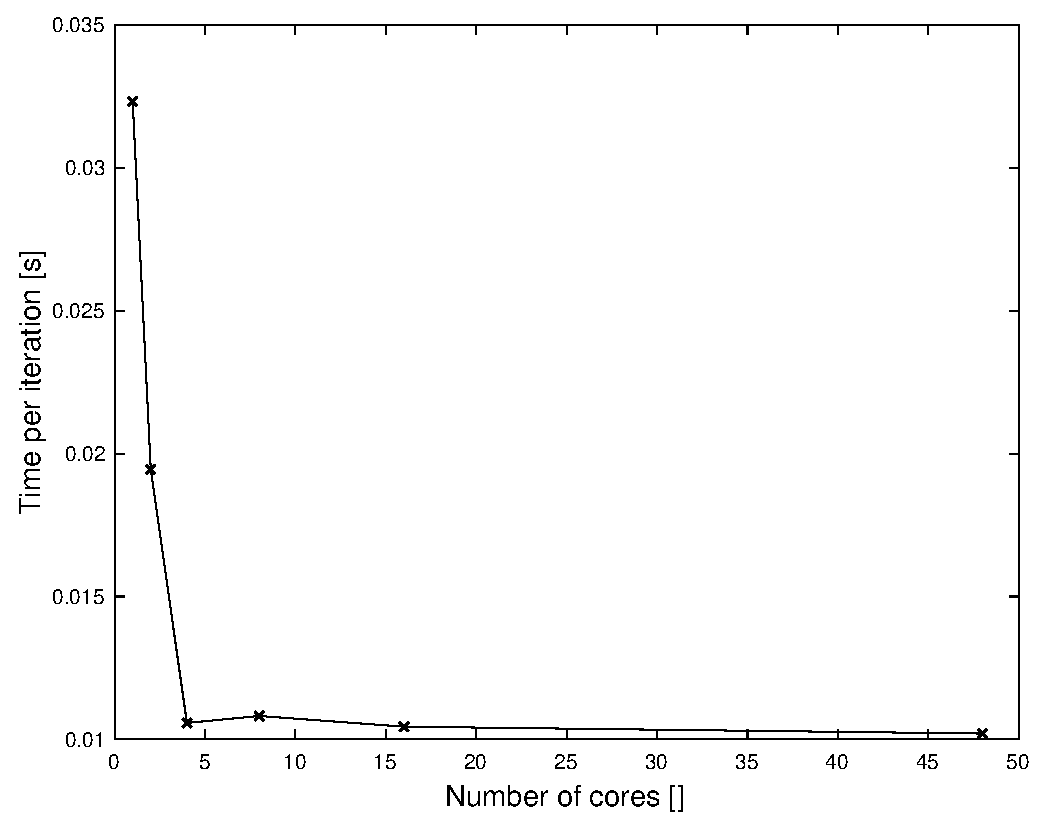
\includegraphics[width=\textwidth]{figures/cores_timeper_256.eps}
%     \caption{\texttt{edge256x192.pgm}}
%     \label{fig:timeper256}
% \end{subfigure}
% \begin{subfigure}[b]{.4\textwidth}
%     \centering
%     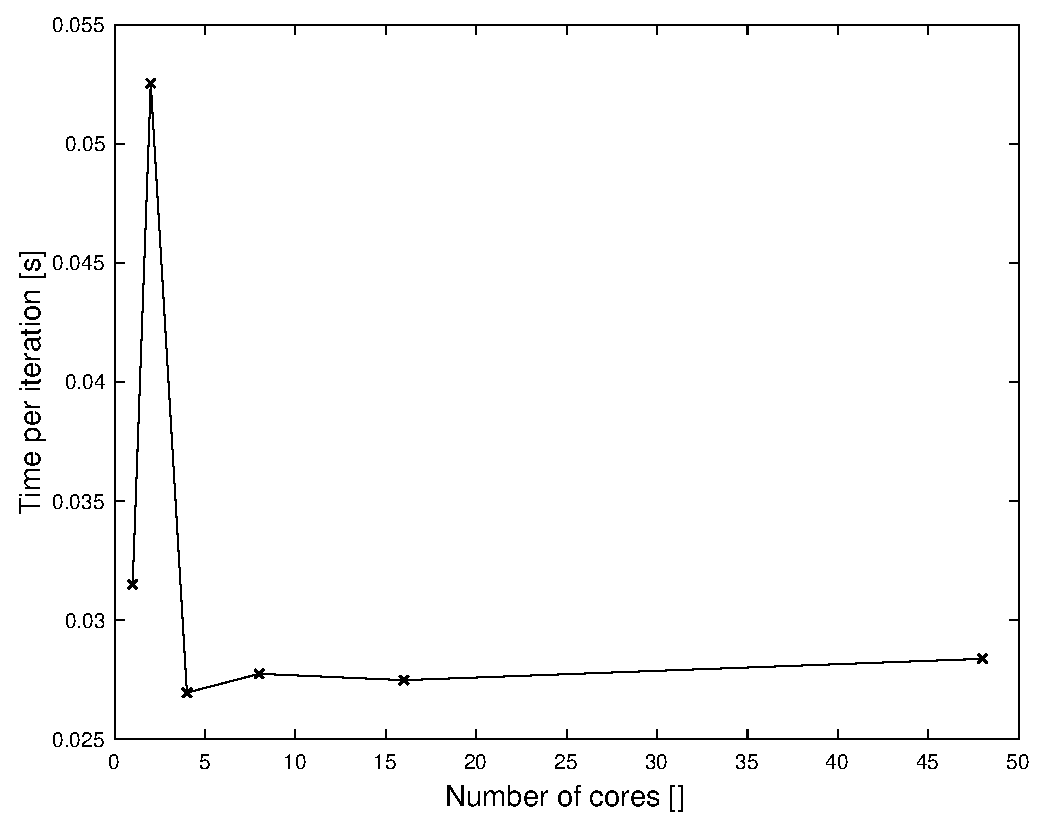
\includegraphics[width=\textwidth]{figures/cores_timeper_384.eps}
%     \caption{\texttt{edge512x384.pgm}}
%     \label{fig:timeper512}
% \end{subfigure}
% \hfill
% \begin{subfigure}[b]{.4\textwidth}
%     \centering
%     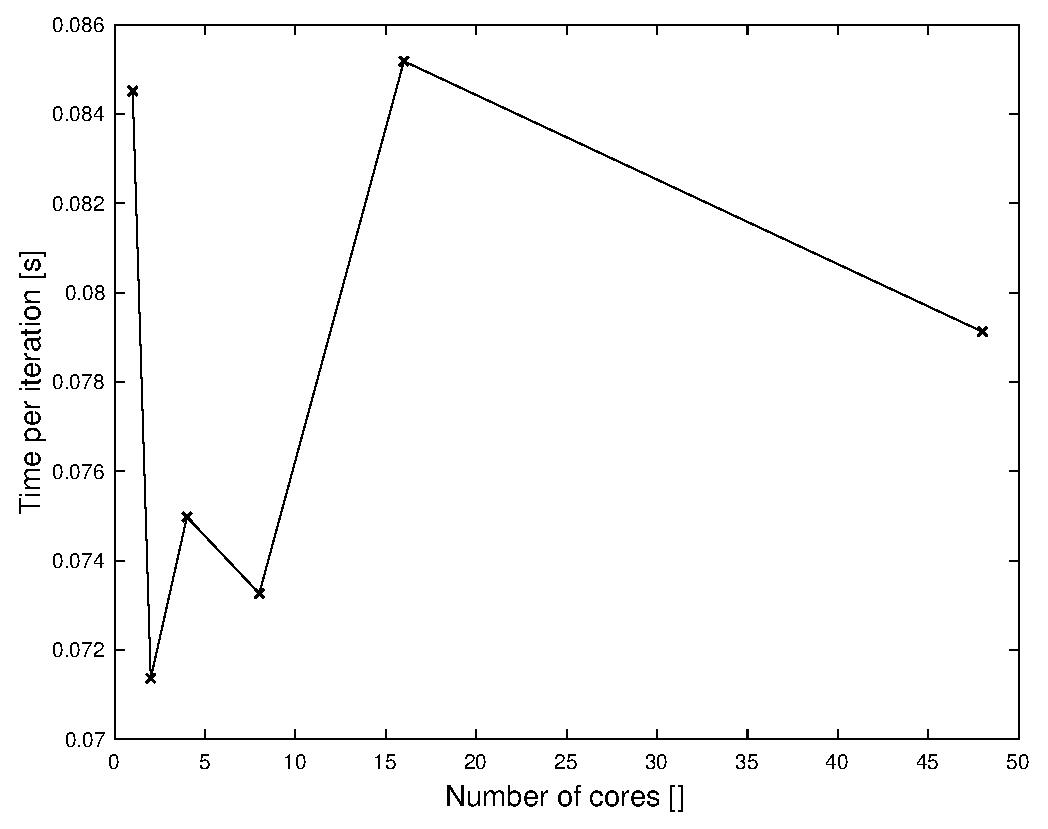
\includegraphics[width=\textwidth]{figures/cores_timeper_768.eps}
%     \caption{\texttt{edge768x768.pgm}}
%     \label{fig:timeper768}
% \end{subfigure}
% \caption{TIME PER, BITCH}
% \label{f:timeper}
% \end{figure}

\section*{Discussion}

Much of the results are as expected, although discrepancies have emerged.

When considering Figure \ref{f:coretime}, we expect to see a quadratic decrease in iteration time, as the local sub-array size decreases in both $M_p$ and $N_p$ with increasing processor count $P$.

However, it's evident that this doesn't occur.
Profiling the program over different core counts reveals that the time required to send the data between processes dominates iteration times for all images across all core counts, with sending times accounting for up to 40\% of iteration timings.

Since it's not possible to directly analyse the amount of time spent sending data and the iteration time together -- timing the data sends requires the use of a \texttt{MPI\_BARRIER} construct which will arbitrarily slow the iteration time -- we can only estimate the impact of the send time on iteration timings. Similarly, creating two different versions of the program does not guarantee reproducibility, with both the compiler potentially performing different optimisations, and the job management system assigning different nodes, with different bandwidths between them.

However, as is expected, the send time increases with core count for all images, with the difference in timings due to varying image sizes being largely insignificant (the bandwidth for ARCHER reported by a simple ping-pong code is far higher than the total volume of data being sent).
It's therefore possible that the iteration performance is a trade-off between the time required to send the data between all processors, and the increase in performance made by having each worker compute a progressively smaller chunk of the overall image.
Figure \ref{f:shares} lends some weight to this theory: while the send and receive methods will not produce the same timings as the \texttt{SCATTERV} and \texttt{GATHERV} constructs, it is clear that the amount of time spent performing data transfers, as a proportion of program run-time, increases with core count. We could therefore expect, particularly for the smaller images, where the relatively fixed sending overhead will dominate performance, that increasing core counts may be accompanied by a counter-intuitive increase in iteration time.
This does indeed appear to be the case in (a) and (c) in Figure \ref{f:coretime}.

\begin{figure}
\begin{subfigure}[b]{.4\textwidth}
    \centering
    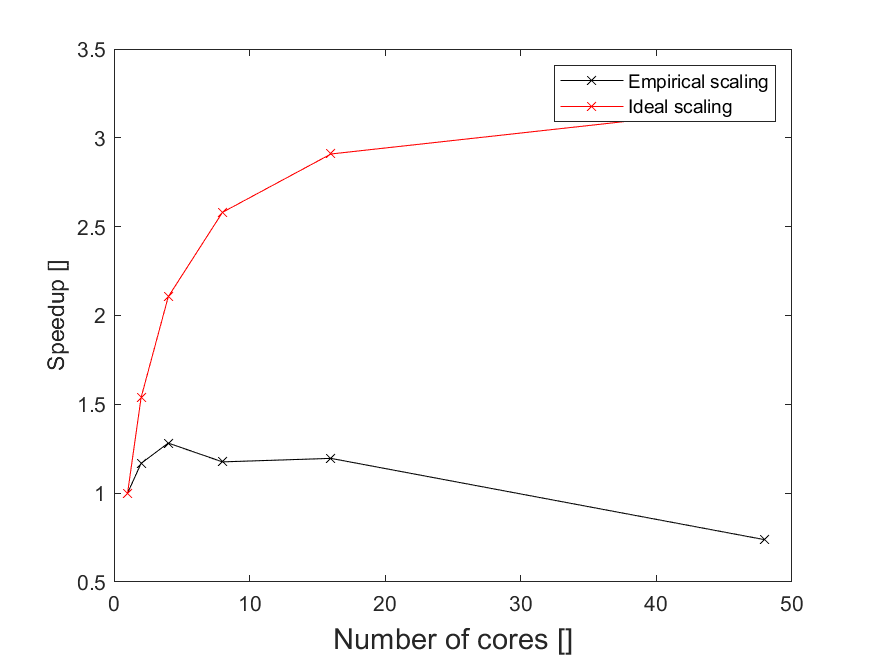
\includegraphics[width=\textwidth]{figures/speedup_198.png}
    \caption{\texttt{edge198x162.pgm}}
    \label{fig:speedup198}
\end{subfigure}
\hfill
\begin{subfigure}[b]{.4\textwidth}
    \centering
    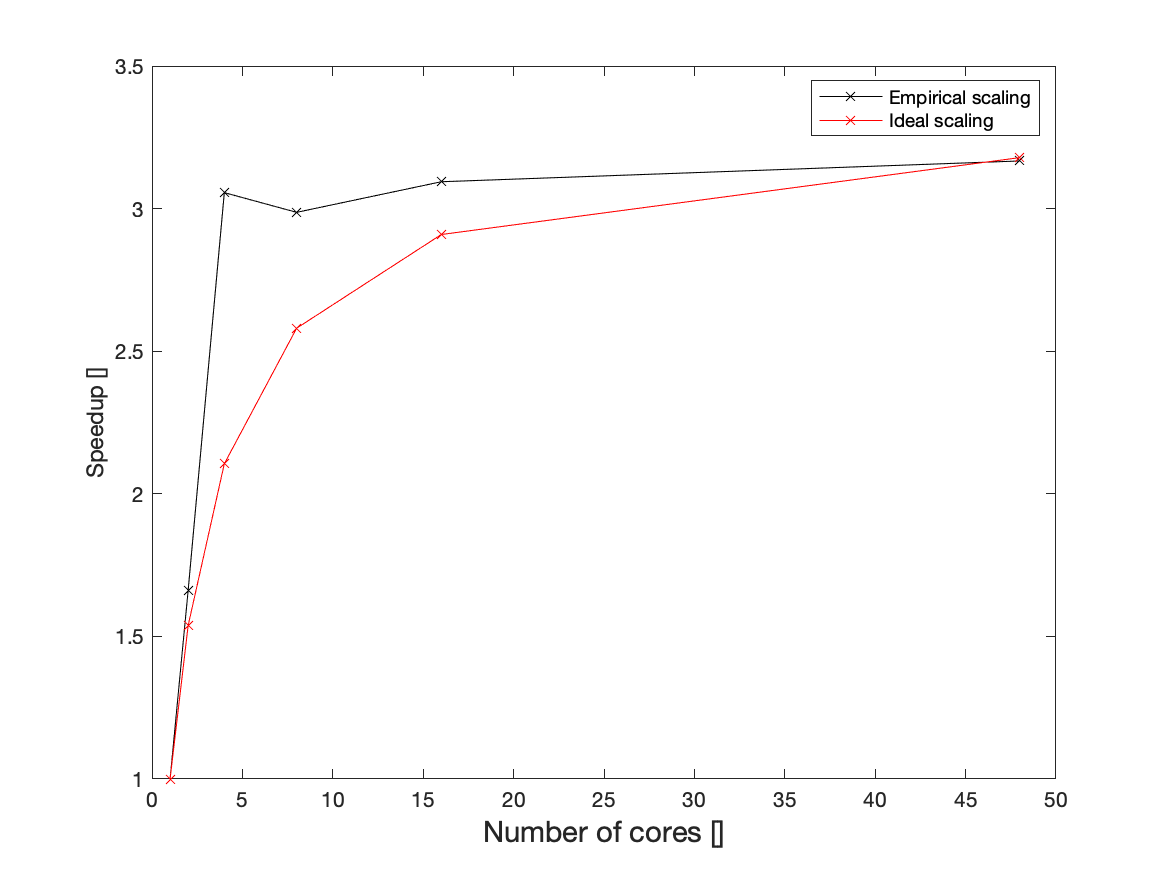
\includegraphics[width=\textwidth]{figures/speedup_256.png}
    \caption{\texttt{edge256x192.pgm}}
    \label{fig:speedup256}
\end{subfigure}
\begin{subfigure}[b]{.4\textwidth}
    \centering
    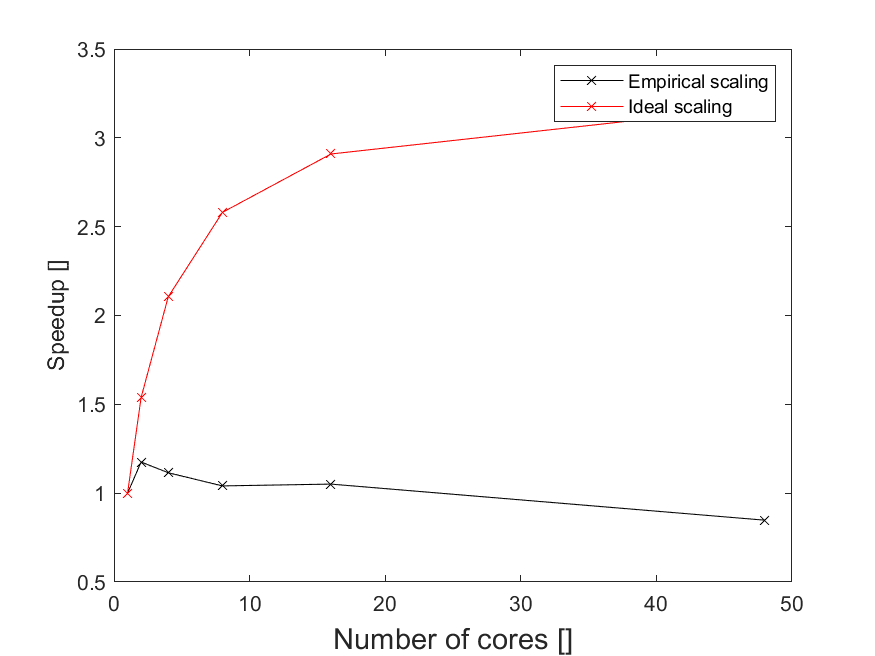
\includegraphics[width=\textwidth]{figures/speedup_384.png}
    \caption{\texttt{edge512x384.pgm}}
    \label{fig:speedup512}
\end{subfigure}
\hfill
\begin{subfigure}[b]{.4\textwidth}
    \centering
    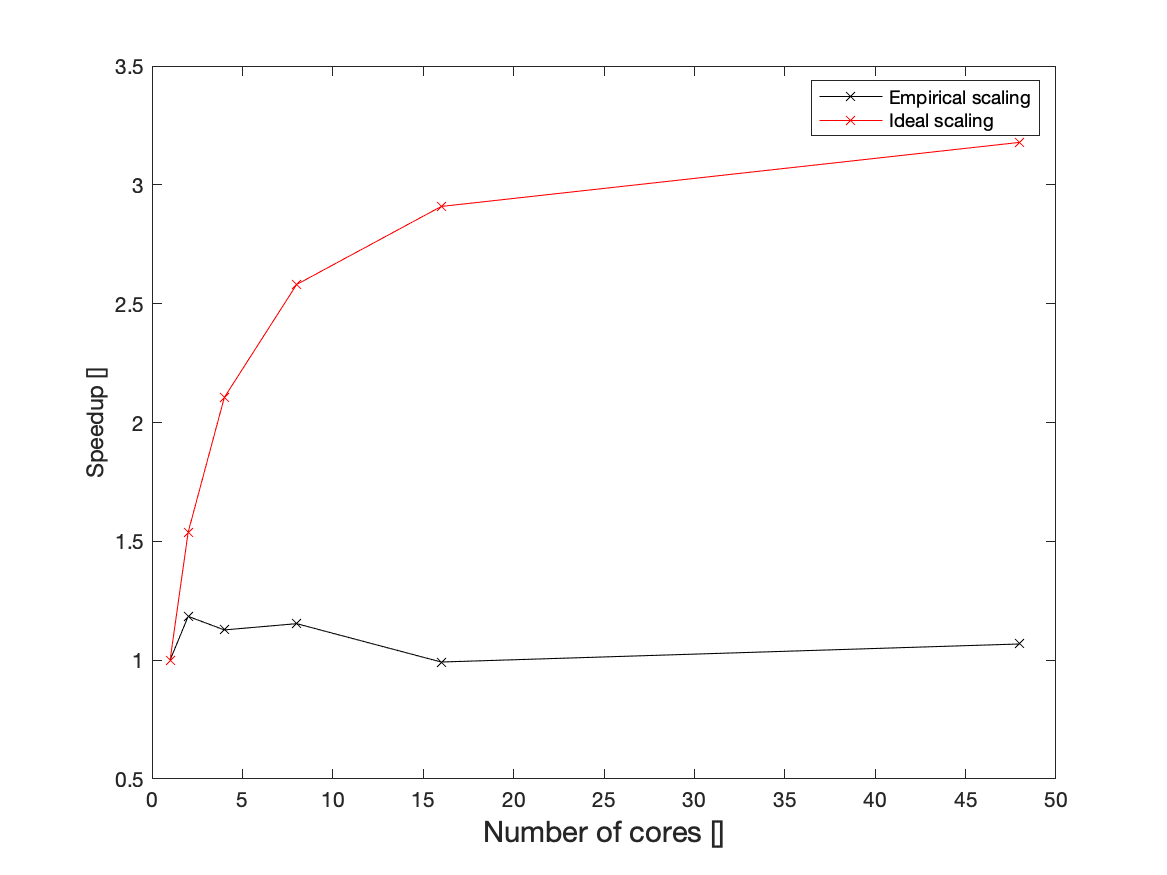
\includegraphics[width=\textwidth]{figures/speedup_768.png}
    \caption{\texttt{edge768x768.pgm}}
    \label{fig:speedup768}
\end{subfigure}
\caption{Ideal scaling against empirical scaling: note that we gain (seemingly) greater than ideal scaling as a result of poor performance for $P=1$.}
\label{f:speedup}
\end{figure}

While this may begin to explain the trends in the data presented in Figure \ref{f:coretime}, it does not explain the large increases in execution time present fir 4 and 16 cores in (d) in the Figures.
Initial assessment would categorise these points as outliers and discard them accordingly, but multiple runs of the program, all on the same node, were performed to be able to reject `outlier behaviour' in the data.

Further profiling would be appropriate to locate the source of the deviation from expected behaviour, but given that (d) provides the timings for the largest image, it would not be unsurprising for the behaviour to be different: here, the iteration time is likely to be far higher compared to data sending (which will, in itself, be higher than normal owing to the greater number of data contained within the horizontal and vertical vectors used for the halo swapping.)

It is also not unreasonable for the performance to be characterised by the frequency of convergence checks; since this operation requires multiple reduction operations, the greater the number of convergence checks, the greater the iteration time. For all of the run-times presented here, the check frequency was kept constant. However, for larger core counts it is again likely that there will be a far greater influence from this step on the overall computation time.

The strong scaling presented in Figure \ref{f:speedup} -- that is, the change in performance for a fixed total problem size with increasing core counts -- shows the scaling is generally very poor.
The ideal scaling, computed using Amdahl's law with a semi-empirical value of $p = .7$ and $s$ equal to the core count, is superimposed on each of the figures.

It is clear that the performance shown by the algorithm is sub-standard. 
Again, it is important to note that performance appears to increase beyond ideal as a result of poor performance from the case where $P = 1$.
There are a number of possible reasons why the scaling is not as expected: many of them have been discussed above. 
In general, while 70\% of the algorithm is parallelisable, it is not possible for all of these portions to be parallelised, and the time taken to transfer halos between nodes, as well as the reductions for the convergence checking, will all prevent the realisation of ideal scaling.
Data transfers also take finite time to compute, which is not assumed in Amdahl's law.

Interestingly, however, we do recover generally good scaling for the \texttt{256x192} image, despite the results of the other images. It could be that this image happens to strike the correct balance between the image processing and the MPI overheads, but the exact reason is unclear.
After two cores, however, the speedup for this image is also limited.
Again, proper profiling would allow the reasons behind this to potentially be uncovered.

\begin{figure}
\begin{subfigure}[b]{.4\textwidth}
    \centering
    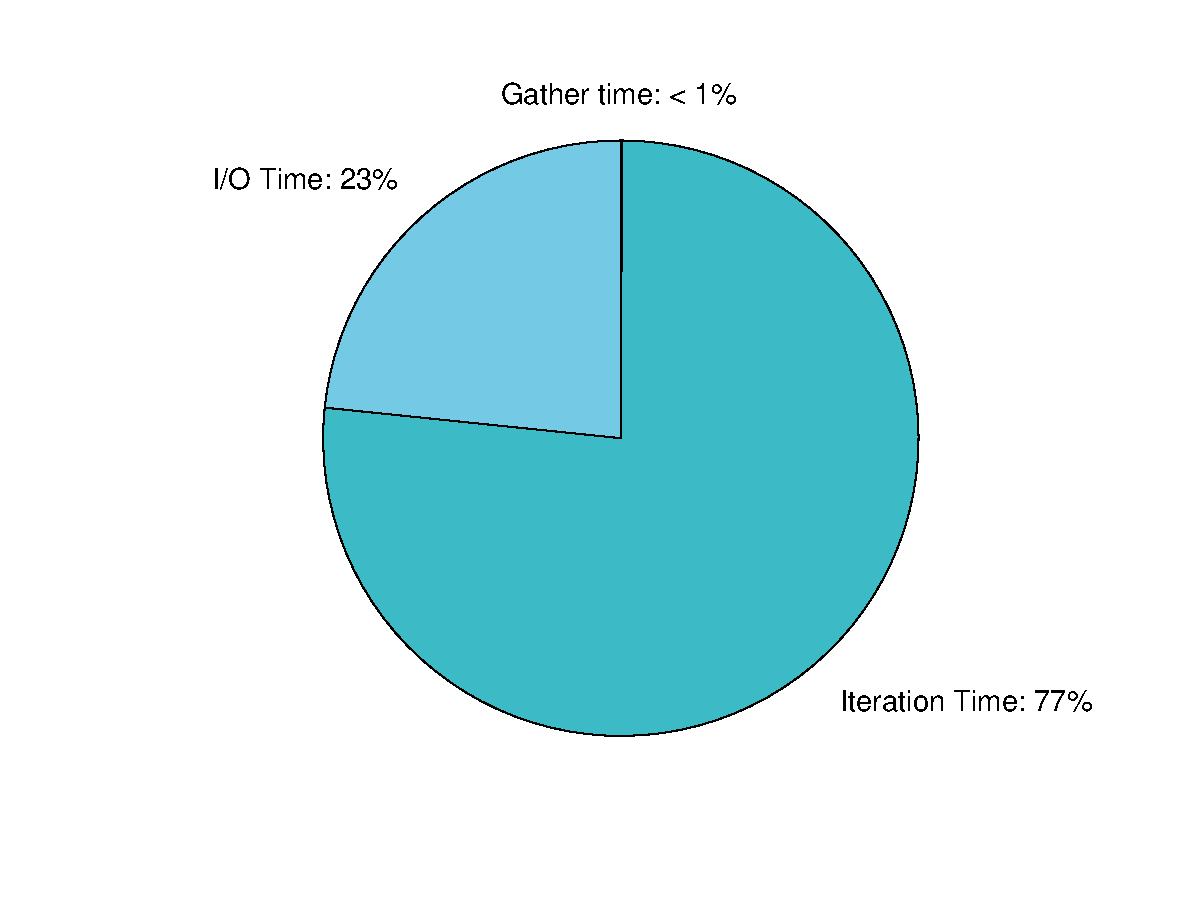
\includegraphics[width=\textwidth]{figures/shares198_1.eps}
    \caption{\texttt{edge198x162.pgm}}
    \label{fig:shares1}
\end{subfigure}
\hfill
\begin{subfigure}[b]{.4\textwidth}
    \centering
    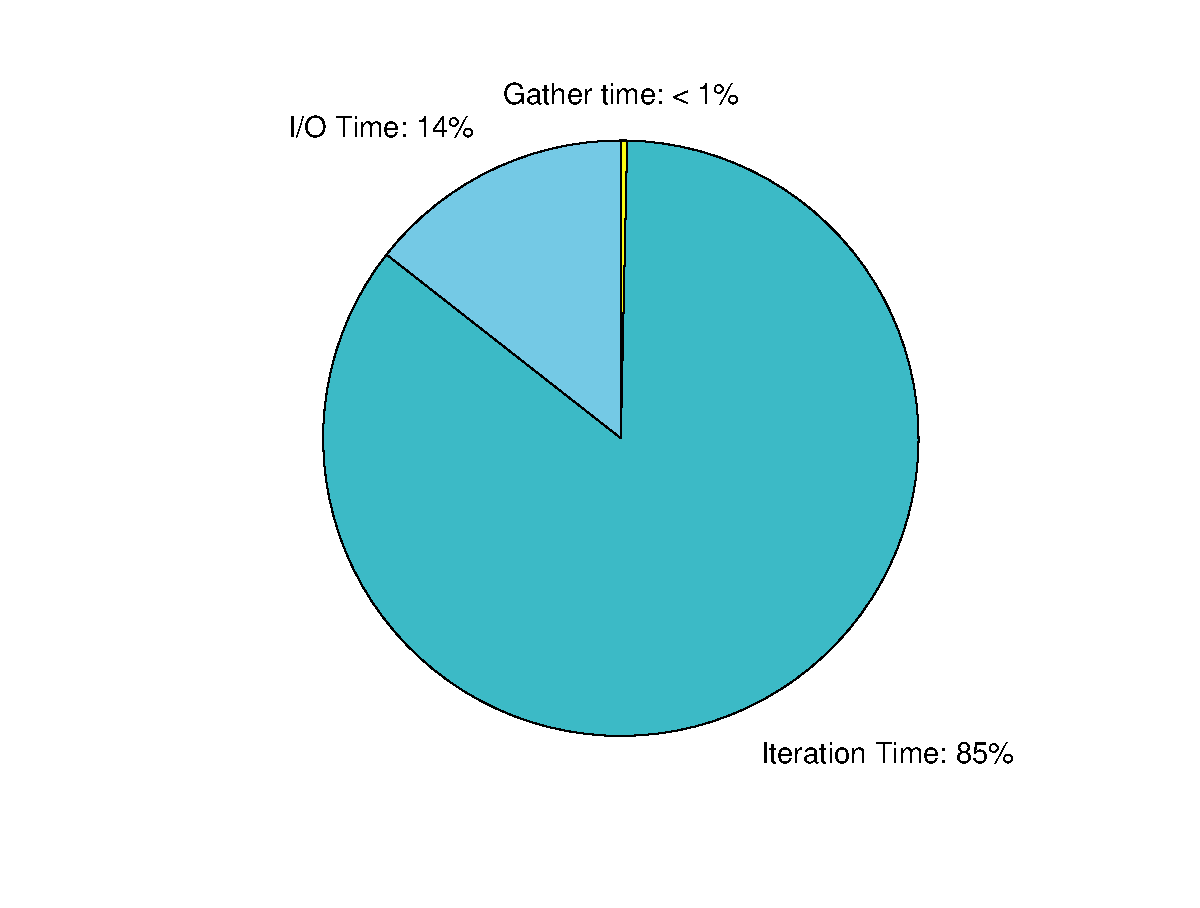
\includegraphics[width=\textwidth]{figures/shares198_2}
    \caption{\texttt{edge256x192.pgm}}
    \label{fig:shares2}
\end{subfigure}
\begin{subfigure}[b]{.4\textwidth}
    \centering
    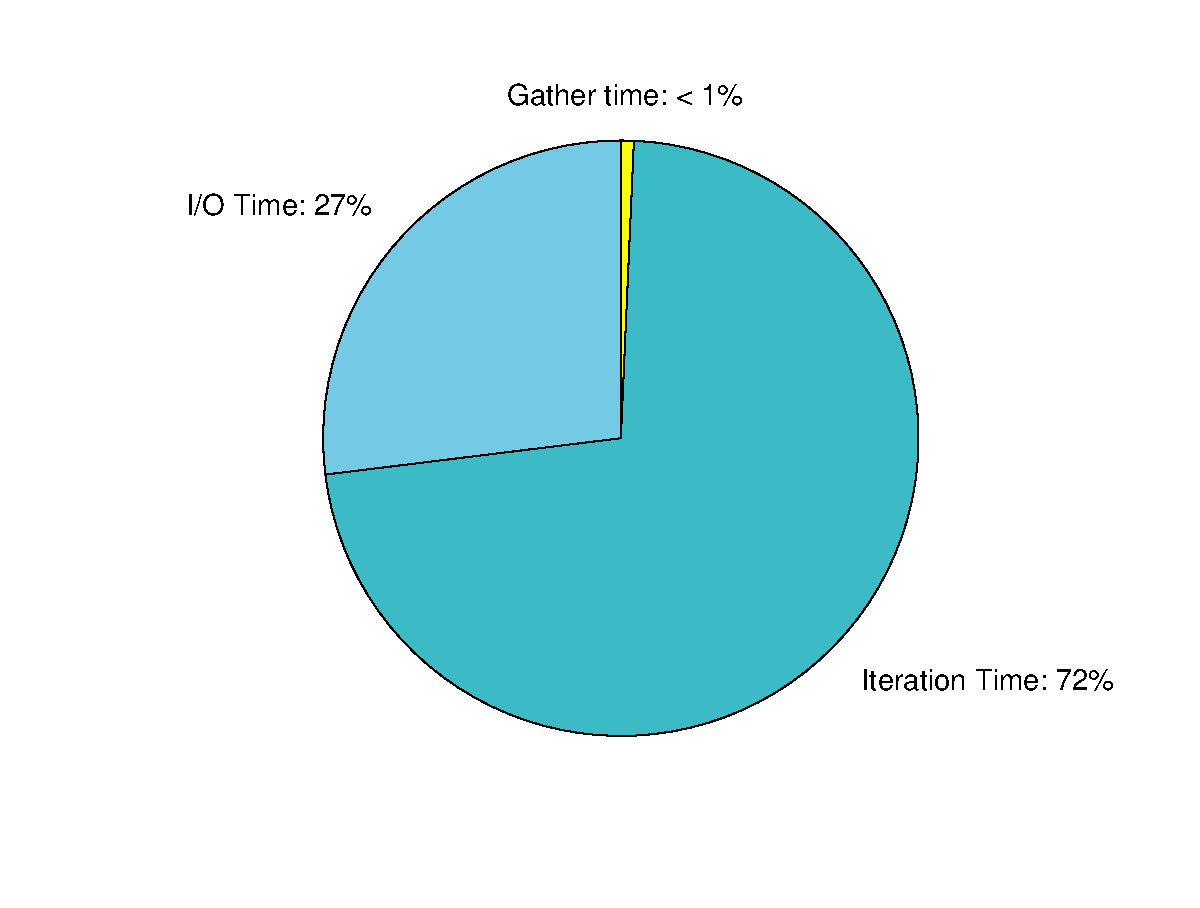
\includegraphics[width=\textwidth]{figures/shares198_4}
    \caption{\texttt{edge512x384.pgm}}
    \label{fig:shares4}
\end{subfigure}
\hfill
\begin{subfigure}[b]{.4\textwidth}
    \centering
    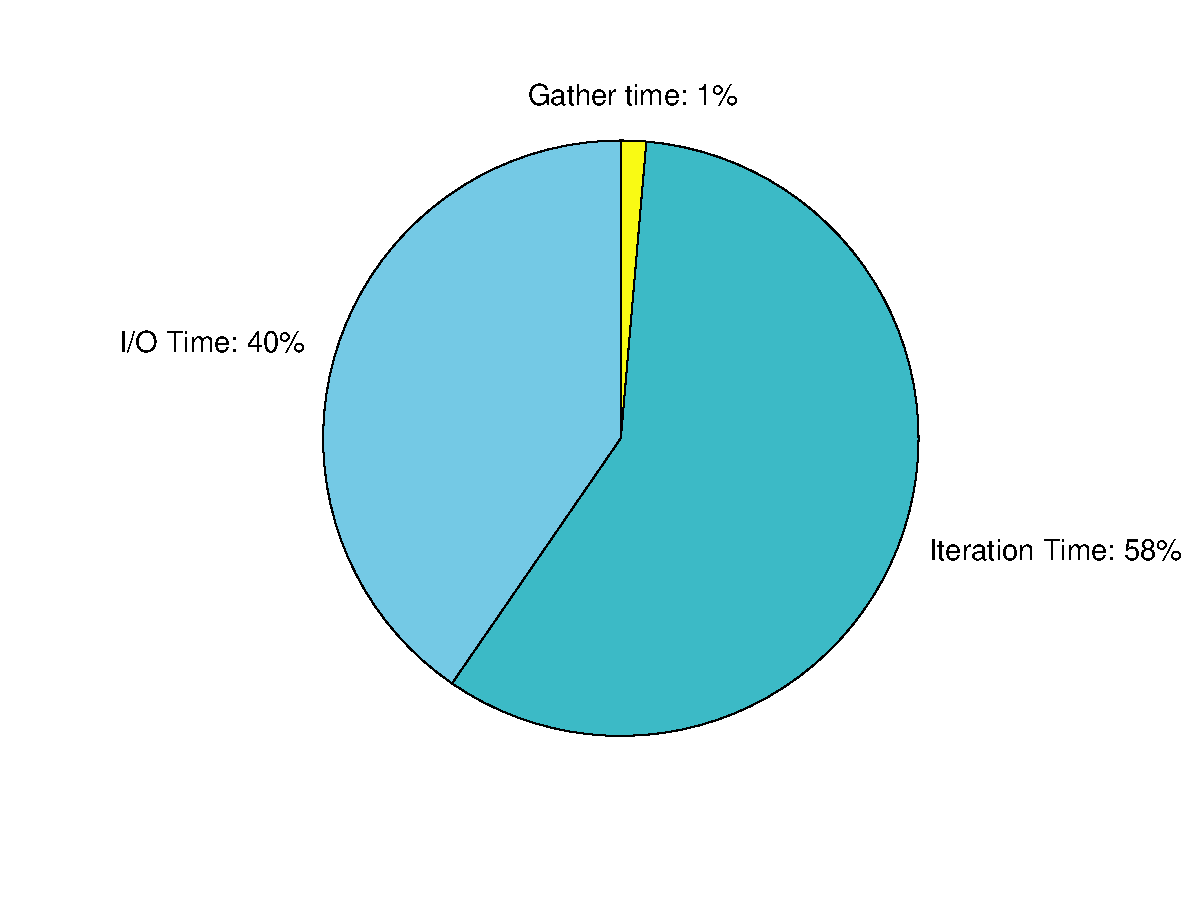
\includegraphics[width=\textwidth]{figures/shares198_8}
    \caption{\texttt{edge768x768.pgm}}
    \label{fig:shares8}
\end{subfigure}
\begin{subfigure}[b]{.4\textwidth}
    \centering
    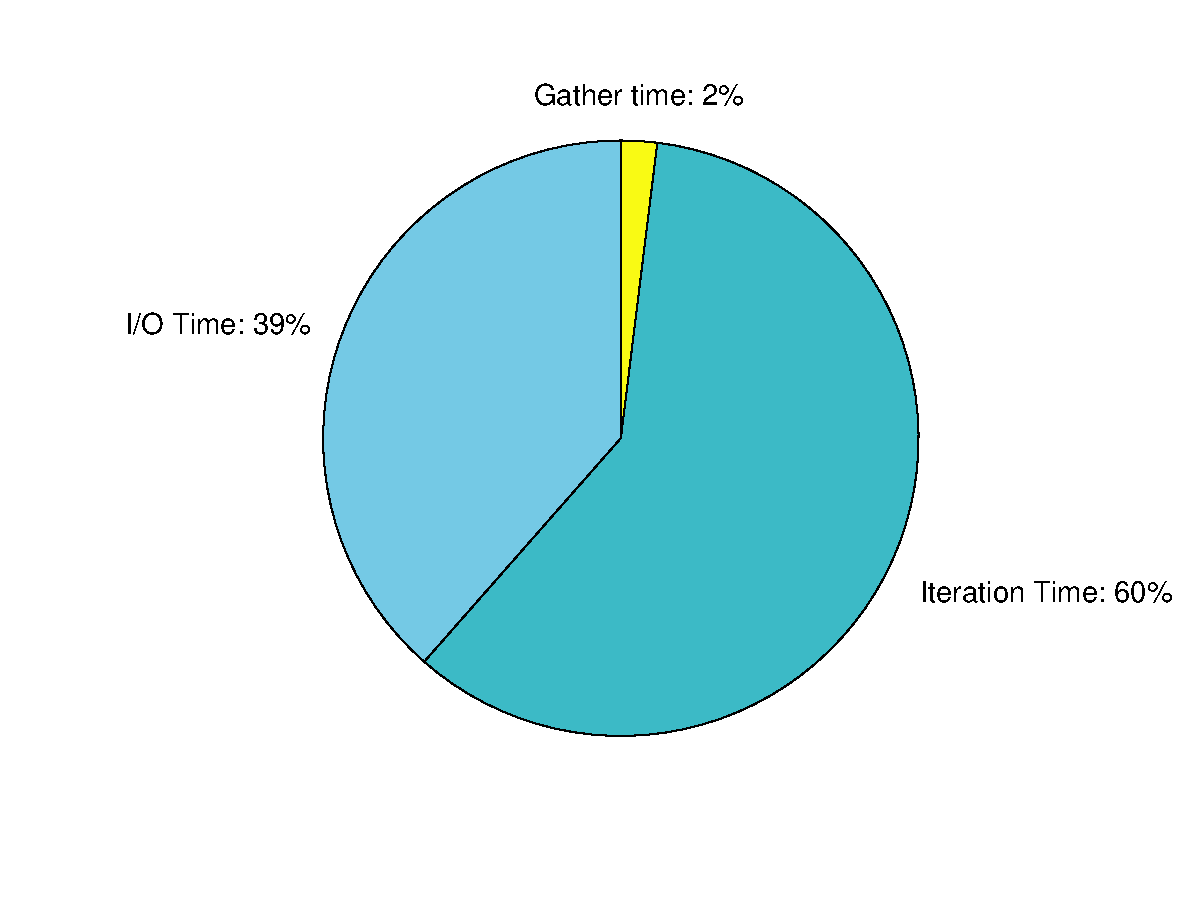
\includegraphics[width=\textwidth]{figures/shares198_16}
    \caption{\texttt{edge512x384.pgm}}
    \label{fig:shares16}
\end{subfigure}
\hfill
\begin{subfigure}[b]{.4\textwidth}
    \centering
    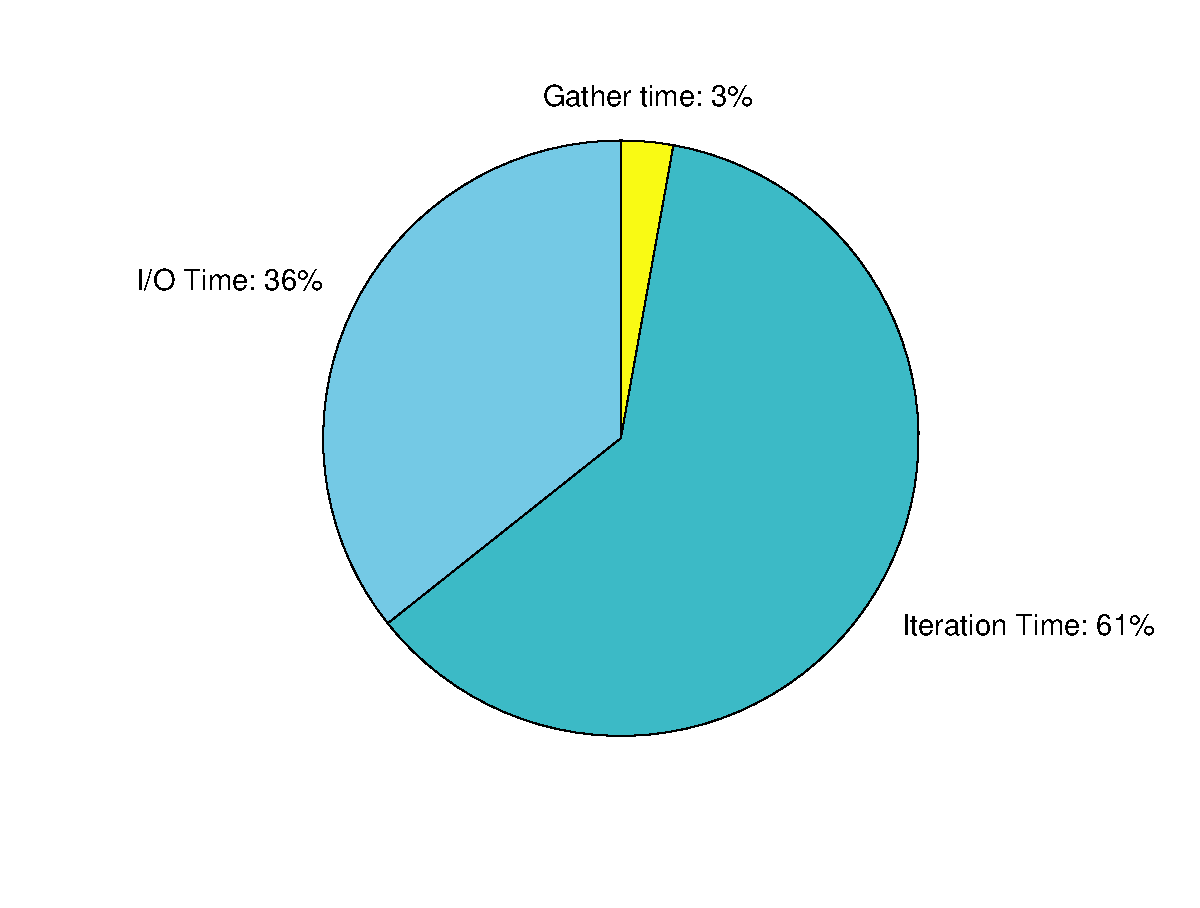
\includegraphics[width=\textwidth]{figures/shares198_48}
    \caption{\texttt{edge768x768.pgm}}
    \label{fig:shares48}
\end{subfigure}
\caption{Time spent by each program in various portions of the code. Interestingly, while the iteration time will decrease for increasing core counts, the increased time to perform the initial scattering and final gathering, will hamper the overall performance of the algorithm.}
\label{f:shares}
\end{figure}

\section*{Discussion: Send and Receive Methods}

When considering the performance of the algorithm, it is also important to justify many of the algorithmic decisions made when designing the program.

In this case, it is important to discuss the send and receive methods implemented. The `final' version of the program uses the \texttt{MPI\_Issend} and \texttt{MPI\_IRecv} for non-blocking communication. 
However, one other sending option exists: \texttt{MPI\_Isend}.
Both are non-blocking -- which is appropriate for their use here, as stated earlier -- but the difference between them lies in when they signal to MPI that the send buffer can be used again:

\begin{itemize}
    \item \tp{MPI\_Isend} returns control either when the data has been copied locally in a buffer owned by the MPI library, or when the data has actually been sent;
    \item \tp{MPI\_ISsend} doesn't buffer data locally and control is returned only after the data has been transferred.
\end{itemize} 

\noindent In any case, both methods were implemented, and their performance measured, and \tp{MPI\_ISsend} had lower execution times for all images, across all metrics, than \tp{MPI\_Isend}.

\section*{Potential Algorithm Improvements}

The performance of the algorithm, while generally better with increasing core numbers, still leaves a lot to be desired.
Changes to the algorithm, or the method used, could result in greater performance increases.

For example, modifying the problem so that there is no dependency on shared halo regions would remove much of the communication overheads present in the current program; this would most likely be performed by changing the underlying method used in the re-construction of the target image, such as by using a discrete Poisson solver \citep{Perez2016}.

Furthermore, it would be worthwhile to experiment with the use of different stopping criteria, in order to perform the least work possible: while the threshold for the difference between two iterations is adjustable in the \tp{problem\_constants} file, other convergence metrics, and ones which do not require the use of a global reduction, could be investigated. The current methodology, if applied carefully, may also still function when applied to a single chunk rather than by performing the reduction.

The use of MPI-I/O on a parallel file system (such as the one present on ARCHER) may also help to combat the \~30\% of the program run-time spent in distributing and receiving the image data file.
However, the use, and implementation of, MPI-I/O is outside the scope of this work.

The use of \tp{MPI\_ALLREDUCE} when computing the convergence checks also has a major impact on the performance of the algorithm; use of another, non-blocking method, may help to improve performance.

\section*{Conclusion}

This report has investigated the performance of a two-dimensional Cartesian topology when applied to a set of sample images on the ARCHER supercomputing cluster. As can be seen with the results presented herein, there are many factors to consider when attempting to increase the performance of a parallel algorithm. In particular, performance is often a balance between gains due to parallelism, and the losses from their related overheads. The results here have shown poor scaling for sample images, although it is important to note that the results may be inappropriate when being considered at such short run-times. The processing of far larger images, which will naturally increase the processing times, may produce far more reliable and accurate timings than those presented here.

\bibliographystyle{plainnat}
\bibliography{bib.bib}

\end{document}
